\documentclass[12pt]{ouparticle}
%\documentclass[11pt,halfline,a4paper,nonnumbib]{ouparticle}

\usepackage[no-math]{fontspec}
\setmainfont{Linux Libertine O}

\graphicspath{{images/}}

\usepackage{langsci-gb4e}%\noautomath
\let\eachwordone=\itshape
\usepackage[textsize=small,backgroundcolor=white]{todonotes}
\usepackage{soul}


\usepackage{booktabs}
\usepackage{multirow}
\newcolumntype{P}[1]{>{\centering\arraybackslash}p{#1}}
\newcolumntype{M}[1]{>{\centering\arraybackslash}m{#1}}
\newcolumntype{L}[1]{>{\raggedright\arraybackslash}p{#1}}
\usepackage{makecell}


\usepackage{xspace}

\usepackage[width=0.8\textwidth]{caption}

\usepackage{natbib}
\bibpunct[:~]{(}{)}{,}{a}{}{,}
\newcommand{\BIBand}{\&}
\setlength{\bibsep}{0pt}
\setlength{\bibhang}{2em}
\bibliographystyle{glossa}
\renewcommand{\bibsection}{}
\newcommand\namecite{\citet}
\newcommand\citeboth{\citealt}
\newcommand{\quotecite}[1]{\citeauthor{#1}'s (\citeyear{#1})}
\renewcommand\cite{\citep}

\newcommand{\high}{\textsc{high}\xspace}
\newcommand{\low}{\textsc{low}\xspace}
\newcommand{\level}{\textsc{level}\xspace}
\newcommand{\gloss}[1]{\textsc{\lowercase{#1}}}
\newcommand{\gl}[1]{\textsc{\lowercase{#1}}}
\newcommand{\REF}[2][]{(\ref{#2}#1)}
\newcommand{\tabref}[1]{Table~\ref{tab:#1}}
\newcommand{\figref}[1]{Figure~\ref{fig:#1}}
\newcommand{\from}{\textless\xspace}

\usepackage{hyperref}
%\hypersetup{toclink=all}


\makeatletter
\newenvironment{Abstract}
    {\list{}{\listparindent 0em%
    %\setlength{\leftmargin}{<value>} adjust if you need
    \itemindent\listparindent
    \rightmargin\leftmargin
    \parsep\z@ \@plus\p@
    }%
    \item\relax}
    {\endlist}
\makeatother



\usepackage{fancyhdr}
\pagestyle{fancy}
\fancyhf{}
\fancyhead[R]{\thepage}

\usepackage{lineno}
\linenumbers

\linespread{1.25}

\usepackage{xcolor}

\usepackage{indentfirst}

\title{Quasi-phonemic vowels in Ampenan Sasak: An acoustic study}

\begin{document}

\maketitle

\begin{abstract}

The allophonic variation between the phonetically-similar tense and lax mid-vowels [e], [ɛ], [o], and [ɔ] varies across dialects. In Ampenan Sasak, traditional documentation and analytical methods based on auditory perception reveal allophonic patterns in alternations of tenseness among mid-vowels. However, words deviate from these patterns in several minimal pairs and in some borrowings. This study analyzes the phonetic properties of mid-vowels through an acoustic analysis of the F1 and F2 of 2,448 vowel tokens. Results suggests that mid-vowels are largely predictable among non-borrowed vocabulary. In final syllables, syllable weight serves as a predictor for the tenseness of mid-vowels. In penultimate syllables, syllable weight has no effect on the tenseness of the vowel. Rather, the tenseness of penultimate mid-vowels is predictable based on the height of the final-syllable vowel. In consideration of both elicitation and acoustic evidence, this paper adopts a descriptive approach by stating that Sasak mid-vowels are largely predictable with some exceptions. However, the paper questions whether all sounds must be identified as a ‘phoneme’ or an ‘allophone’ and argues that quasi-phonemic segments are a valuable intermediate category for both phonological theory and language documentation. 


\end{abstract}

\newpage

%% pacs numbers not used

%  End of title page for Preprint option --------------------------------- %

\subsection{Introduction}\label{sec:introduction}

Despite the widespread accessibility and portability of high-quality audio recorders and tools for acoustic analysis, phonetic analysis is generally not a topic of focus in grammatical descriptions, and phonological descriptions of under-documented languages remain largely perception-based \citep{maddieson2002}. Researchers' judgments --- which are generally based on results of word elicitation and the determination of whether segments occur in free variation or complementary distribution --- have been the primary means employed by field linguists for determining phonemic segments and their allophones. Sketches largely describe regular phonological patterns and only briefly mention areas of uncertainty, if at all; yet, these areas of uncertainty have revealed the existence of intermediate phonological relationships \footnote{Intermediate phonological relationships have been called various names throughout the literature, some of which include semi-phonemic, quasi-contrastive, weak contrast, and partial contrast \citep{hall2013}.} in several languages \citep{hall2013}. This paper uses the term quasi-phonemes  to describe segments that behave like both phonemes and allophones; sometimes they occur in predictable \footnote{Predictability in this context refers to segments that occur in complimentary distribution. Unpredictable segments are those that exist in free variation}  environments, and sometimes they do not (i.e. minimal or near-minimal pairs). Quantitative analysis of acoustic data is valuable to further identify and understand such gradient phenomena. Further, by minimizing the unavoidable subjectivity of researchers' perceptual impressions, acoustic analysis is particularly useful in distinguishing patterns between perceptually-similar segments whose relationship may be difficult to disentangle when relying on traditional elicitation methods. This paper identifies quasi-phonemic patterns in Sasak, an under-documented language of Indonesia, and describes them in detail through the use of acoustic analysis.


Mid-vowels in a dialect of Sasak referred to in this paper as Ampenan Sasak present an interesting environment for acoustic study because of the unclear phonemic status of the mid-vowels, [e, o, ɛ, ɔ], that occur even cross-dialectally \citep{chahal1998, jacq1998, archangeli2018}. In Ampenan Sasak, mid-vowels present an apparent contradiction. Tense vs. lax vowels largely occur in complementary distribution based on syllable weight; however, there are a few occurrences of minimal pairs between back mid-vowels. This paper aims to expand this current knowledge about Sasak mid-vowels by conducting an acoustic analysis of F1 and F2 values to further elucidate the vowel inventory of Ampenan Sasak, which has yet to be phonetically or phonemically analyzed. 2,455 tokens of systematic occurrences of mid-vowels were collected from seven female speakers of Ampenan Sasak. The formant values of these vowel productions were analyzed and modeled in order to answer two prevailing questions: 1) Can variations in mid-vowels in final position be explained by differences in syllable weight? and 2) Are penultimate vowels also sensitive to syllable weight, and to what extent are they sensitive to the quality of the vowel in the final syllable? The study addresses these questions by eliciting a systematically-chosen wordlist containing mid-vowels preceding each possible coda in Sasak. Speakers completed a production task to produce each word in a sentence context, and the f1 and f2 of vowels in final and penultimate syllables were analyzed using Linear Mixed Effects Models (LMEM).

To contextualize this study, Sasak and previous phonetic and phonological study on the language are first introduced before further investigation into its vowel system is undertaken.


\section{Ampenan Sasak and its segmental system}\label{sec:segment}

The Sasak language is spoken by approximately 3 million people on the eastern Indonesian island of Lombok \citep{eberhard2019}. The language is closely related to Balinese and Sumbawan and is part of a proposed Malayo-Sumbawan subgrouping of the Western Malayo-Polynesian branch of Austronesian \citep{adelaar2005}. While Sasak has a still-thriving population, fewer children are learning the language as the Sasak-speaking population becomes a globally-oriented populace \citep{djenar2018}. Sasak as a whole has received much academic attention in the form of dictionaries \citep{thoir1985, staff1995}, grammars \citep{thoir1985/6}, and journal articles \citep{austin2010, archangeli2017}; however, Ampenan Sasak has not yet been studied by researchers.

Traditionally, researchers have distinguished dialects by their deictic terms for ‘like this’ and ‘like that.’ The five major dialects are called Ngeno-ngene, Nggeto-nggete, Meno-mene, Kuto-kute, and Meriaq-meriku. Figure \ref{fig:sasak_dialects}, originally presented in \citet{jacq1998}, illustrates their distribution. Yet, whether this is the most appropriate categorization of Sasak dialects is still contested \citep{austin2012, jacq1998}. Researchers have observed phonetic and sometimes phonological variation within the Meno-mene variety, spoken in central Lombok \citep{archangeli2018,chahal1998,jacq1998,teeuw1958}.

\begin{figure}[h!]
    \centering
    \caption{The geographic distribution of Sasak dialects. Ampenan Sasak is a Ngeno-ngene variety spoken west of Mataram \citep{jacq1998}.}.
    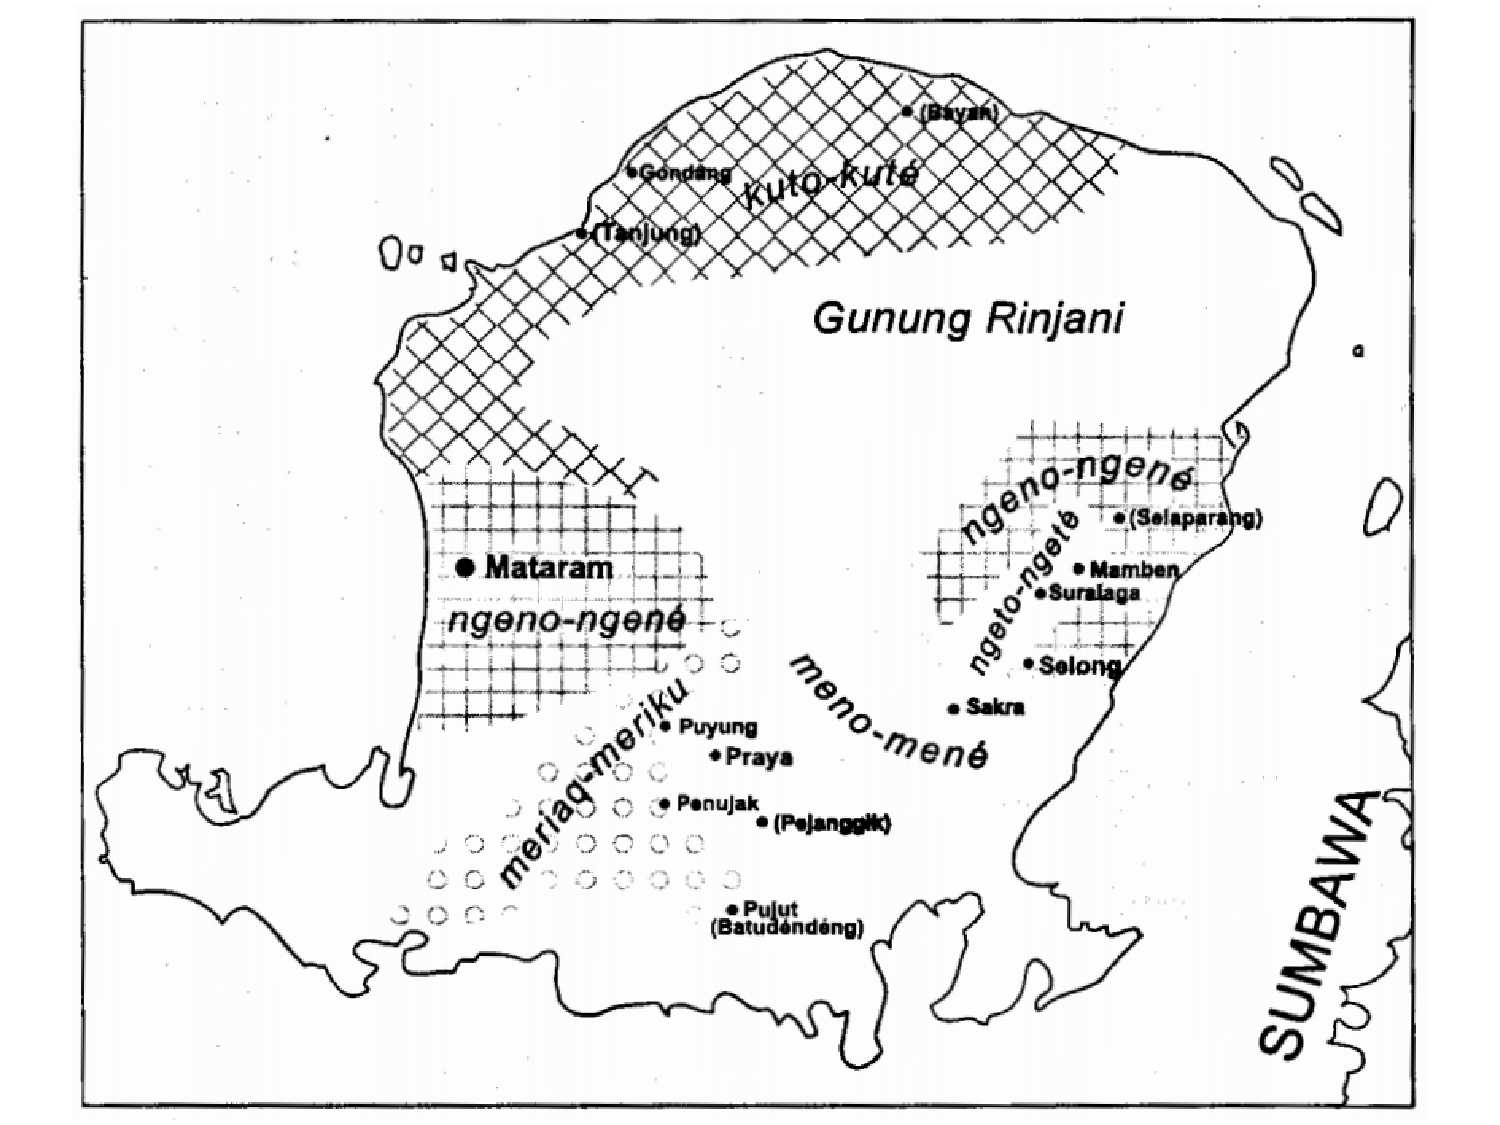
\includegraphics[width=0.75\textwidth]{Figure1.pdf}
    \label{fig:sasak_dialects}
\end{figure} 


Ampenan Sasak is a Ngeno-ngene variety spoken in Ampenan, an urban subdistrict of Lombok's capital city, Mataram. The dialect situation in Mataram is not yet understood, but Ampenan Sasak was named as such to delineate that the dialect is different from Ngeno-ngene. While Ampenan Sasak has not been previously recognized by researchers, people living in Ampenan have identified that their Sasak is different --- both phonetically and syntactically --- from that spoken in other parts of the city; yet even within Ampenan, there is linguistic variation. This data is from Pondok Perasi, a coastal suburban neighborhood that is defined by its fishing economy. Because of the evident yet little-understood linguistic variation, this paper does not make claims about the Ngeno-ngene dialect of Sasak as a whole.


Ampenan Sasak has a typical phoneme inventory of an Indonesian language. Table \ref{tab:sasak_consonants} shows the consonant inventory of Ampenan Sasak. If the orthographic representation does not match the phonetic symbol, it is noted in brackets <>. 

\begin{table}[ht]
\centering
\caption{Ampenan Sasak Consonant Inventory based on elicitation with a native speaker}
\label{tab:sasak_consonants}
%\begin{ruledtabular}
\begin{tabular}{l | l l l l l l l}
	& Bilabial  & Alveolar & Post-alveolar & Palatal & Velar & Glottal  \\
\hline
Stop & p b & t d & & & k g & ʔ <’> \\
Nasal & m & n & & ɲ <ny> & ŋ<ng> &\\
Tap/Trill & & r & & & & & \\
Fricative & & s & & & & h \\
Affricate & & & tʃ <c> dʒ <j> & & & \\
Lateral & & l & & & & & \\
\end{tabular}
%\end{ruledtabular}
\end{table}

\begin{figure}[h!]
	  \centering
	  \caption{The Ampenan Sasak vowel inventory based on elicitation with a native speaker. Phonemes are unmarked, and allophones are in square brackets. Mid-vowels are in gray because of their unclear phonemic status.}
	  \label{tab:sasak_vowels}
      \begin{tikzpicture}[scale=2]
        \tikzset{
    vowel/.style={fill=white, anchor=mid, text depth=0ex, text height=1ex},
    dot/.style={circle,fill=black,minimum size=0.4ex,inner sep=0pt,outer sep=-1pt},
        }
        \coordinate (hf) at (0,2); % high front
        \coordinate (hb) at (2,2); % high back
        \coordinate (lf) at (1,0); % low front
        \coordinate (lb) at (2,0); % low back
        \def\V(#1,#2){barycentric cs:hf={(3-#1)*(2-#2)},hb={(3-#1)*#2},lf={#1*(2-#2)},lb={#1*#2}}

        % Draw the horizontal lines first.
        \draw (\V(0,0)) -- (\V(0,2));
        \draw (\V(1,0)) -- (\V(1,2));
        \draw (\V(2,0)) -- (\V(2,2));
        \draw (\V(3,0)) -- (\V(3,2));

        % Draw the vertical lines.
        \draw (\V(0,0)) -- (\V(3,0));
        \draw (\V(0,1)) -- (\V(3,1));
        \draw (\V(0,2)) -- (\V(3,2));

        % Place the unpaired symbols last, on top of the vertical lines.
        \path (\V(1.5,1))      node[vowel]       {ə};
        \path (\V(0.25,0.25))  node[vowel]       {i};
        \path (\V(0.5,0.5))    node[vowel]       {[ɪ]};
        \path (\V(2.5,1))      node[vowel]       {a};
        \path (\V(0.25,1.75))  node[vowel]       {u};
        \path (\V(0.5,1.5))    node[vowel]       {[ʊ]};
        \path (\V(1.25,1.75))  node[vowel]       {\textcolor{gray}{o}};
        \path (\V(1.65,1.65))    node[vowel]       {\textcolor{gray}{ɔ}};
        \path (\V(1.25,0.25))  node[vowel]       {\textcolor{gray}{e}};        
        \path (\V(1.65,0.45))   node[vowel]       {\textcolor{gray}{ɛ}};        
      \end{tikzpicture}
	    \label{fig:sasak_vowels}
	\end{figure}

Ampenan Sasak’s vowel system, shown in Figure \ref{fig:sasak_vowels} below, is also quite typical of the languages of Indonesia. Based on the author's judgments during elicitation, the lax segments shown in brackets are analyzed to be allophones of the corresponding tense segments.\footnote{In using the terms `tense' and `lax' no claims are made about the physiological properties of the vocal tract as these sounds are being produced. Rather, measurements of F1-F2 are reported as a proxy for tense vs. lax vowels with a higher F1 suggesting a more lax vowel. Based on the results of this study, tense vowels tend to be more peripheral and precise with lower F1 values while lax vowels are more centralized with higher F1 values \citep{wood1975,halle1977}.}  Mid-vowels are in gray to indicate their unclear phonemic status. The distribution of tense/lax for high vowels in the final syllable depends on the weight of that syllable, while the distribution of mid vowels is slightly unclear. Features other than tense/lax are not restricted. Tense vowels tend to occur in open final syllables or those with a glottal stop coda (for terminological convenience, both of these are henceforth considered light syllables, though they could just as well be categorized different). Lax vowels tend to occur in final syllables with any coda excluding the glottal stop (henceforth heavy syllables) \footnote{A linear mixed effects model observing the difference between f2 and f1 formant values shows that vowels in no-coda and glottal stop-coda syllables show no difference (\textit{t = -1.167, p = 0.26291})}. The tense/lax allophonic variation based on syllable structure is clear with high vowels and significantly less clear with mid-vowels. However, the following examples illustrate the general relationship between mid-vowels and syllable structure: [sere] `lemongrass,' [tabeʔ] `excuse me,' [durɛn] `durian,' [jɛŋgɛr] `rooster comb,' [bisoʔ] `wash,' [rebo] `Wednesday,' [jagɔŋ] `corn,' [gubɔk] `village.'

Further, the weight of the final syllable may also serve as a predictor of laxness among penultimate mid-vowels. It appears that when two mid-vowels are in a word, they both have the same tenseness, indicating that there may be a correlation. In [bembeʔ] `goat', although the penultimate syllable is closed, and thus one may expect a lax mid-vowel [ɛ], it contains the tense mid-vowel [e]. Similarly, in the word [gɔɾɛŋ] `fried', although the penultimate syllable is open, the penultimate vowel is lax like the vowel in the final syllable. As these examples depict, this is both possible when the mid-vowels are identical, and when they are different. Several other examples include: [ɛpɛn] `owner,' [tɔkɔl] `sit,'[kɔtɔŋ] 'burnt,' and [ɛlɛh] `drift.' One may thus observe a correlation between the realization of each mid-vowel, that may be a result of vowel harmony. \footnote{In this paper vowel harmony is defined as a collection of properties in which some features of certain segments spread to others \citep{wood1975}.}


However, despite these broad patterns, there are a few  minimal pairs between back mid-vowels which a number of the consultants for this study identified as words in Ampenan Sasak. These are presented in Table \ref{tab:minimal_pairs}. These minimal pairs suggest that back mid-vowels could be considered phonemes, as they may occur in free variation. Minimal pairs between front mid-vowels have yet to be identified. However, perceptually, the vowel quality of front vowels is difficult to determine using traditional auditory analysis, particularly before nasal codas. For instance, based on the author's perceptual impressions, \textit{kepeng} `money' was initially transcribed as [kepeŋ], but \textit{goreng} `fried' has always clearly been pronounced [gɔɾɛŋ]. Whether these words are near-minimal pairs or not is unclear.

\begin{table}[ht]
\caption{Minimal Pairs among back mid-vowels seem to deviate from allophonic patterns seen elsewhere in the language.}
\label{tab:minimal_pairs}
%\begin{ruledtabular}
\begin{tabular}{l|ll|ll}
/o/∼/ɔ/	& /bəɾəmbok/ & `to discuss' & /bəɾəmbɔk/ & `to           breathe'\\
        & 	/koboʔ-an/ &	`leven more'	&  /kɔbɔʔ-an/& `bowl for washing hand while eating’\\
        & /kədok/ & `dig' & /kədɔk/ & `deaf'\\
        & /ros/	& Personal name  & /rɔs/ & Personal name\\
\end{tabular}
%\end{ruledtabular}
\end{table}

Evidently, all minimal pairs occur between /o/ and /ɔ/ before unreleased /k/ or /ʔ/. This raised questions as to whether there was simply allophonic variation between word-final /k/ and /ʔ/ in these instances. However, this was tested by adding the multifunctional suffiix \textit{-an} --- seen in the minimal pairs /koboʔ-an/ and /kɔbɔʔ-an/ --- to the end of each word. In doing so, /k/ is released, clearly indicating the tongue's contact with the velum. This testing revealed that codas were consistent while the vowels varied. 

While the pair of names in Table \ref{tab:minimal_pairs} are likely borrowings, they may represent how borrowings are shaping Ampenan Sasak's phonemic inventory. In addition to the minimal pair distinction between [ros] and [rɔs], borrowed terms, such as [gədoŋ] `building’ and [agostos] `August' provide clear exceptions to predictable allophonic patterns among mid-vowels. The word [gedoŋ] `building', which is apparently borrowed from Indonesian \textit{gedung} with the same meaning, is a near minimal pair with [embɔŋ] `traditional resevoir'. While [embɔŋ] contains a lax mid-vowel in its heavy final syllable, [gedoŋ] contains a tense mid-vowel. Similarly, [agostos] `August', borrowed from Dutch \textit{augustus}, most likely with Indonesian as an intermediary, contains two tense vowels despite the heavy final syllable. Regardless of the word form in the source language, the current Sasak words serve as exceptions to the near-predictability of [e], [ɛ], [o], and [ɔ] .

In addition, many studies have emphasized the importance of acknowledging speaker intuitions in determining whether segments are allophones or phonemes \citep{hualde2005,scobbie2008}. Sasak speakers' perceptions of mid-vowel distinctions are variable. In writing, Sasak speech communities do not distinguish /ə/ from /e/, and /ɛ/, nor do they distinguish /o/ from /ɔ/. The segments /e/, /ɛ/, and /ə/ are all represented by the letter \textit{e}, and /o/ and /ɔ/, are both represented by \textit{o}. In perception, sometimes speakers have very clear intuitions as to which mid-vowel variant is appropriate, and other times, they do not. For example, the primary consultant for this study and a PhD student in linguistics, has stated several times that \textit{bembeq} `goat'  is pronounced [bembeʔ], not [bɛmbɛʔ]. She notes that the latter is how the word would be spoken in central Sasak dialects, and this is consistent with the analysis in \citet[]{chahal1998}. However, such intuitions seem to be lexically specific and are not always consistent both within and across speakers. 

Though determining stress in Ampenan Sasak is beyond the scope of this study, it is worth exploring stress's potential relationship to the current data due to the observed relationship between stress and vowel quality in the region \citep{kaland2019}. Stress has been an engaged area of investigation among Indonesian languages because of the elusive nature of word-level stress using traditional measurements of pitch, intensity, and duration. This has been the case in Sasak; none of the measurements of pitch, intensity, or duration, have revealed any word-level stress patterns. Stress is clearly not contrastive, but primary stress position remains unclear. Native Sasak speakers identify stress to be consistently on the penultimate syllable. This coincides with patterns seen in Austronesian languages in which of those with fixed stress (slightly over half), 80\% have penultimate stress. If Ampenan Sasak does indeed have penultimate stress, this would have no influence on the current data as unstressed (final) syllables are only compared to other unstressed syllables and likewise with stressed (penultimate) syllables. Instead of word-level stress, many Malayo-Polynesian languages exhibit what \citet{goedemans2014} call `phrasal accent,' which has been observed in several dialects of Malay \citep{vanzanten1998, vanzanten2004, maskikit2016}. Likewise phrasal accent would have no bearing on the data, because the clausal context of each word is the same. 

Other Austronesian languages have variable stress due to other (sometimes phonological) factors, such as Papuan Malay, which clearly has penultimate stress when there is no mid-vowel in penultimate syllable \citep{kaland2019}. It is possible that syllable weight drives stress in Sasak, but under the current methodology, it would not be possible to determine whether vowels lower because of syllable weight or because heavy syllables are stressed. In light of the presented data, it is assumed that stress, while possibly interacting with results, would not nullify them.

% Yet stress plays a limited role in the current discussion since final and penultimate vowels are never analyzed together. As such, stressed vowels are only compared to other stressed vowels and vice versa. 

% If this were the case in Sasak, stress would be fixed in each response because each word occurs in the same sentential context.

% while other dialects, such as Papuan Malay, clearly have penultimate stress under certain conditions (when there is no mid-vowel in penultimate syllable) \citep{kaland2019}

\subsection{Previous work}

Studies on Sasak varieties have come to varying conclusions about the relationship between mid-vowels. \citet[5]{chahal1998} analyzes a Meno-mene variety of Sasak and finds that the vowel phonemes include /i, e, a, ə, o, u/. Two factors influence where lax variants appear: weight and stress. Lax vowels appear in closed syllables (syllables with a CVC structure) and tense vowels occur in open syllables (syllables with no coda). Chahal also claims that stress falls on the final syllable of this dialect of Sasak, and in stressed syllables, there is more variation in the pronunciation of the vowel. Finally, Chahal determines that this dialect of Sasak appears to have `bi-directional gradient vowel height harmony' whereby the realization of a vowel in final syllable may affect that of a vowel in penultimate syllable and vice versa \citep[11-12]{chahal1998}.

While both \citet{archangeli2018} and \citet{chahal1998} conclude that the Meno-mene dialect of Sasak has a six-vowel system (/i, e, a, ə, u, o/), the interpretations reached by \citet{archangeli2018} in the distribution of tense and lax vowel segments are not in accordance with those of \citet{chahal1998}. \citeauthor{archangeli2018} find no influence of syllable weight at all, nor do the authors observe vowel harmony. Rather, all influence on vowel quality derives from the stress on the syllable in which it occurs, which according to the authors falls largely on the final syllable. Like Chahal, \citeauthor{archangeli2018} find that vowels occupy a smaller acoustic space in unstressed (i.e., penultimate) syllables than they do in stressed (i.e., final) ones. 

In consideration of both previous studies which grapple with the challenge that tense and lax vowels pose to phonetic and phonological analysis, and of the elicitation data which exhibits several minimal pairs between [o] and [ɔ], mid-vowels are the focus of this study. The study analyzes the production of vowels in systematically elicited sentential contexts and measures their f1 and f2 to target their quality based on environmental factors. The study addresses two primary questions 1) Are mid-vowels in final position sensitive to syllable weight? 2) Are penultimate vowels affected by their own syllable weight, and to what extent are they sensitive to the quality of the vowel in the following syllable? 

The next section details the experimental design and analytical methods of this study.


\section{Analytical Methods}\label{sec:methods}

\subsection{Materials}\label{sec:materials}

Data for this acoustic study were gathered through the elicitation of a measured wordlist that controlled for the syllable and surrounding segments of each mid-vowel. The wordlist contained 81 critical items that did not appear to be loanwords or recent borrowings. They are shared in Appendix A. Items were chosen based on the phonological environment of the vowel in the final syllable including: (1) syllable weight, (2) coda segment, and (3) height of preceding vowel (low, mid, high, schwa). These factors were balanced to the greatest extent possible. When possible, four instances of each final syllable mid-vowel before every possible coda segment were included. Fifteen filler words were also included to assure that the data contained all vowels in the phoneme inventory in both penultimate and final position.

\newpage

% \begin{table}[ht]
% \centering
% \caption{The number of each coda segment following final-syllable mid-vowels in the data set.}
% \label{tab:CodaSeg}
% %\begin{ruledtabular}
% \begin{tabular}{l | l l}
% Coda & e & o \\
% \hline
% q & 4 & 4\\
% h & 4 & 3\\
% n & 2 & 4\\
% ng & 4 & 4\\
% p & 3 & 0\\
% t & 4 & 3\\
% s & 2 & 3\\
% l & 2 & 3\\
% r & 4 & 2\\
% k & 3 & 3\\
% 0 & 4 & 4\\

% \end{tabular}
% %\end{ruledtabular}
% \end{table}

Because of the limitations of the data and more broadly, Sasak phonotactics, for the purposes of investigating vowel harmony, penultimate mid-vowels could not occur before every vowel in final position. In this dataset /o/ only occurred before /a/ when the /a/ was in a heavy syllable while /e/ only occurred before /a/ when /a/ was in a light syllable. There were no instances of mid-vowels preceding a schwa or a high vowel, and schwa only occurred in heavy final syllables.

\subsection{Procedure}\label{sec:procedure}

Words in this wordlist were presented via a slideshow on a laptop computer. Figure \ref{fig:kemos} provides an example of the format of each slide. The Sasak word appeared in the center of the screen. Practical Sasak orthography as used by speakers does not have diacritics. As a result, the pronunciation of a word may be ambiguous since the segments /e/, /ɛ/, and /ə/ are all represented by the letter \textit{e}, and /o/ and /ɔ/, are both represented by \textit{o}. To eliminate any ambiguity, each slide also includes the Indonesian translation below the Sasak word. Since all speakers were bilingual in Sasak and Indonesian, the Indonesian translation effectively disambiguated any Sasak homographs. At the suggestion of the primary consultant for this study, slides were one of three colors: red (\textit{beaq}), green (\textit{ijo}), and yellow \textit{(kuning}). For the example in Figure \ref{fig:kemos}, speakers were instructed to say “‘kemos’ is red,” or \textit{kemos warna beaq}, in Sasak.  This presentation format captured each critical word in a sentence, leading to a more natural pronunciation of the word. The order of the words and the colors associated with each word were entirely random. Each word was repeated once, resulting in a total of 162 word productions for each participant. Speakers could proceed through the task at their own pace. They were able to repeat the word or response if they wanted.

\begin{figure}[ht]
    \centering
    \caption{Example of experimental slide: The large word \textit{kemos} is the Sasak word. The smaller word beneath is the Indonesian translation. The background is red. The expected response is \textit{Kemos warna beaq} `Kemos is red.'}
    
\includegraphics[width=0.75\textwidth]{Figure3.jpg}
    \label{fig:kemos}
\end{figure}

Throughout the task, participants wore a lapel microphone that recorded a digital .wav file recorded at 44.1 kHz/16 bit on Zoom H2 solid state recorder in order to capture high-quality acoustic data. Participants were additionally filmed with a FullHD Panasonic video camera and the internal cardioid microphone of the Zoom H2 recorder in order to capture the environment as well as the participants’ facial movements and gestures as they completed the task. Recordings were completed at the speaker’s home or at that of their neighbors. Often several women completed the task in the same session. All data is archived in the Kaipuleohone Language Archive at the University of Hawai'i at Mānoa.

\subsection{Participants}\label{sec:participants}

Seven female speakers of Sasak aged 18-45 participated in this study. All speakers grew up speaking Ampenan Sasak and were bilingual in Indonesian. 

\subsection{Acoustic Measurements}\label{sec:measurements}
Each critical word and the vowel onset and offset were segmented using Praat \citep{boersma2019}. The F1 and F2 was then measured at the mid-point of the vowel. Vowel spaces were normalized across speakers using the vowel-extrinsic formula presented by the Lobanov method of vowel normalization. This method was chosen because it is a well-attested method for factoring out physiological differences between speakers. Further, the Lobanov method works well with datasets that measure the entire vowel space within a single dialect. Finally, plots depicting vowels normalized by the Lobanov method closely resemble regular F1-F2 plots, facilitating presentation and analysis \citep{adank2004}.

\subsection{Statistical Analysis}\label{sec:analysis}
The lme4 package in R was used to fit linear mixed-effects models (LMEM) to the data \citep{bates2014}. In total, four models were fitted to the data which addressed two primary questions 1) Are mid-vowels in final position sensitive to syllable weight? 2) Are penultimate vowels affected by their own syllable weight, and to what extent are they sensitive to the quality of the vowel in the following syllable? The models investigating the effect of syllable weight on vowel quality had either the F1 or F2 of the final-syllable vowel as the dependent variable, with fixed effects of \textsc{segment} and syllable \textsc{weight}. 

Models used to investigate vowel harmony effects were fitted to the F1 and F2 values of penultimate syllable vowels respectively with two interactions as independent variables -- penultimate \textsc{segment}*\textsc{height} of of the final syllable segment and penultimate \textsc{segment}*\textsc{weight} of the penultimate syllable segment. These two interactions were included to answer two pertinent questions 1) Does the weight of the penultimate syllable have an effect on the F1 or F2 of the vowel? 2) Does the height of the final syllable vowel affect the F1 or F2 of the penultimate vowel (e.g., does a lax vowel in final syllable cause the F1 of the penultimate vowel to increase)? 

All models also included vowel \textsc{duration} as a simple effect with no interactions (Moon \& Lindblom 1994). Further, random intercepts of \textsc{speaker} and \textsc{word} were included in all models. Due to data sparsity, none of the models included random slopes as they did not converge. With the recommendations of \citeauthor{barr2013} (2013), the models were as detailed as possible while still being able to converge.

Sections 3.1 and 3.2 present results that address syllable weight effects on final syllable vowels, and Section 3.3 presents results that address whether vowel harmony is occurring in penultimate vowels.


\section{Results}\label{sec:results}

\subsection{F1 and F2 by Final Syllable Weight}\label{sec:Syll1f1_SegWeight}

Table \ref{tab:Syll2f1_SegWeight} displays the table of coefficients from the LMEM fitted to the F1 values of vowels in final syllables. This model includes the normalized F1 as the dependent variable and syllable \textsc{weight}, \textsc{segment}, and \textsc{duration} as independent variables. The results reveal significant interactions between /e/ and syllable weight and between /o/ and syllable weight. When the syllable weight is light, the F1 is significantly lower than that of a vowel in a heavy syllable for both /e/ (\textit{t = -6.422, p < .001}) and /o/ (\textit{t = -6.762, p < .001}). /i/, /u/ and /a/ do not show the same effect of syllable weight on F1. Figure \ref{fig:stats_f1_final} visualizes this effect. Notable in this figure is the stark difference between mid-vowels /e/ and /o/ in heavy and light syllables.

\begin{table}[h!]
\centering
\caption{The table of coefficients for F1 of final syllable vowels. Independent variables include \textsc{segment}, \textsc{syllable weight}, and \textsc{duration}. Random intercepts include \textsc{speaker} and \textsc{word}. Mid-vowels show highest variation due to syllable weight.}
\label{tab:Syll2f1_SegWeight}
%\begin{ruledtabular}
\begin{tabular}{l | r r r r r}
Effect & Est. & SE & df & t & p-value\\
\hline
(Intercept) &    1.059   &  0.174  & 8.85  &  6.102 & .000\\
Weightlight  &   -0.024  &  0.118  & 433.1  &  0.21 &  .8.34 \\ 
e       &      -0.808     &  0.081  & 133.6 & -9.963 & <.001\\
i       &      -2.025    &  0.12   & 131 & -16.840 & <.001\\
o       &     -0.808     &  0.079  & 140.1 & -10.1609 & <.001\\
u       &      -1.896    &  0.128  & 122.1  & -14.77 & <.001\\
Duration &     <.001        &  <.001  & 1041  & 0.664    & .507\\
Weightlight x e & -0.889  &  0.138  & 281 & -6.422 & <.001\\
Weightlight x i & 0.124   &  0.212  & 101.9 & -0.582  & .562    \\
Weightlight x o & -0.929  &  0.137  & 252.4   & -6.762 & <.001\\
Weightlight x u & 0.121   &  0.261  & 79.56  & -0.462  & .645 \\

\end{tabular}
%\end{ruledtabular}
\end{table}

% \begin{table}[h!]
% \centering
% \caption{The table of coefficients for F1 of final syllable vowels. Independent variables include \textsc{segment}, \textsc{syllable weight}, and \textsc{duration}. Random intercepts include \textsc{speaker} and \textsc{word}. Mid-vowels show highest variation due to syllable weight.}
% \label{tab:Syll2f1_SegWeight}
% %\begin{ruledtabular}
% \begin{tabular}{l | r r r r r}
% Effect & Est. & SE & df & t & p-value\\
% \hline
% (Intercept) &   \textit{1.059}   &  \textit{0.174}  & \textit{8.85}  &  \textit{6.102} & \textit{.000}\\
% Weightlight  &   \textit{-0.024}  &  \textit{0.118}  & \textit{433.1}  &  \textit{0.21} & \textit{ n.s.} \\ 
% e       &      \textit{-0.808}     &  \textit{0.081}  & \textit{133.6} & \textit{-9.963} & \textit{<.001}\\
% i       &       \textit{-2.025}    &  \textit{0.12}   & \textit{131} & \textit{-16.840} & \textit{<.001}\\
% o       &     \textit{-0.808}     &  \textit{0.079}  & \textit{140.1} & \textit{-10.161} & \textit{<.001}\\
% u       &       \textit{-1.896}    &  \textit{0.128}  & \textit{122.1}  & \textit{-14.77} & \textit{<.001}\\
% Duration &  \textit{<.001 }       & \textit{<.001}  & \textit{1041}  & \textit{0.664}    & \textit{n.s.}\\
% Weightlight x e & \textit{-0.889}  &  \textit{0.138}  & \textit{281} & \textit{-6.422} & \textit{<.001}\\
% Weightlight x i & \textit{0.124}   &  \textit{0.212}  & \textit{101.9} & \textit{-0.582}  & \textit{n.s.}    \\
% Weightlight x o & \textit{-0.929}  &  \textit{0.137}  & \textit{252.4}   & \textit{-6.762} & \textit{<.001}\\
% Weightlight x u & \textit{0.121}   &  \textit{0.261}  & \textit{79.56}  & \textit{-0.462}  & \textit{n.s.} \\

% \end{tabular}
% %\end{ruledtabular}
% \end{table}


\begin{figure}[h!]
    \centering
    \caption{Model outputs of the F1 of final vowel segments as influenced by final syllable weight. Mid-vowels show the greatest effects.}
    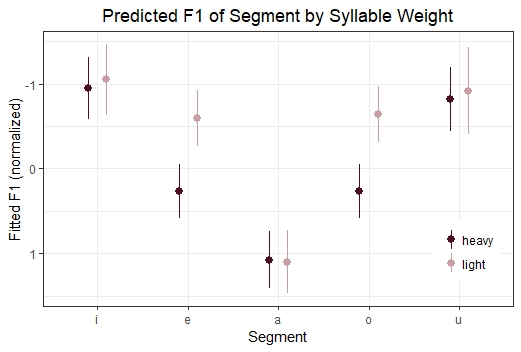
\includegraphics[width=0.75\textwidth]{Figure5.jpg}
    \label{fig:stats_f1_final}
\end{figure}

\newpage

Table \ref{tab:Syll2f2_SegWeight} displays the table of coefficients from a second LMEM fitted to the F2 values of vowels in final syllables. This model was identical to the first model except that the dependent variable was the normalized F2 values. This model shows that F2 is only distinctly different as a result of syllable weight among the back vowels /u/ (\textit{t = -3.965, p = .000}) and /o/ (\textit{t = -3.129, p = 0.002}). /a/ also shows this distinction (\textit{t = 2.28, p = 0.029}), but it shows the reverse trend than is seen among back vowels. /a/ in light syllables tends to have a higher F2 than in heavy syllables while the F2 of back vowels in light syllables tends to be lower than in heavy syllables. While there is not significant interaction between weight and segment among front vowels, they show the same pattern as /a/ in which F2 is slightly higher in light syllables than in heavy syllables. Figure \ref{fig:stats_f2_final} exhibits the results observed as a result of this model. /u/ and somewhat less so /o/ show a visually-distinct difference based on syllable weight.

\begin{table} [h!]
\centering
\caption{The table of coefficients for F2 of final syllable vowels. Independent variables include \textsc{segment}, \textsc{syllable weight}, and \textsc{duration}. back-vowels show highest variation due to syllable weight.}
\label{tab:Syll2f2_SegWeight}
%\begin{ruledtabular}
\begin{tabular}{l | r r r r r}
Effect & Est. & SE & df & t & p-value\\
\hline
(Intercept)    & -0.286 & 0.089 & 69.31 & -3.233 & .002 \\
Weightlight    & 0.275  & 0.124  & 448.8 &  2.209 & .029  \\
e              & 1.015  & 0.084   & 154.8 & 12.091 & <.001 \\
i              & 1.631  &  0.124  & 146.6 & 13.117 & <.001 \\
o              & -0.549 & 0.082  & 161.7  & -6.665 & <.001 \\
u              & -0.372 & 0.132  & 140.9    & -2.806 & .006 \\
Duration       & <-.001 & <.001  & 907.2824.3  & 1.432 & .152\\
Weightlight x e &  .115  & .145  & 306.5  &  0.793  & 0.428   \\
Weightlight x i &  -.023 & .219  & 122  &  -0.105 & .916   \\
Weightlight x o & -.451  & .144  & 180.8  & -3.129  & .002\\
Weightlight x u & -1.057  & .267  & 96.32  & -3.965  & .000 \\
\end{tabular}
\end{table}

% \begin{table} [h!]
% \centering
% \caption{The table of coefficients for F2 of final syllable vowels. Independent variables include \textsc{segment}, \textsc{syllable weight}, and \textsc{duration}. back-vowels show highest variation due to syllable weight.}
% \label{tab:Syll2f2_SegWeight}
% %\begin{ruledtabular}
% \begin{tabular}{l | r r r r r}
% Effect & Est. & SE & df & t & p-value\\
% \hline
% (Intercept)    \textit{ & -0.286 & 0.089 & 69.31 & -3.233 & .002 }\\
% Weightlight     \textit{& 0.275  & 0.124  & 448.8 &  2.209 & .029}  \\
% e               \textit{& 1.015  & 0.084   & 154.8 & 12.091 & <.001} \\
% i               \textit{& 1.631  &  0.124  & 146.6 & 13.117 & <.001} \\
% o               \textit{& -0.549 & 0.082  & 161.7  & -6.665 & <.001} \\
% u              \textit{ & -0.372 & 0.132  & 140.9    & -2.806 & .006} \\
% Duration     \textit{& <-.001 & <.001  & 907.2824.3  & 1.432 & n.s.}\\
% Weightlight x e \textit{&  .115  & .145  & 306.5  &  0.793  & n.s.}   \\
% Weightlight x i \textit{&  -.023 & .219  & 122  &  -0.105 & n.s.}   \\
% Weightlight x o \textit{& -.451  & .144  & 180.8  & -3.129  & .002}\\
% Weightlight x u \textit{& -1.057  & .267  & 96.32  & -3.965  & .000} \\
% \end{tabular}
% %\end{ruledtabular}
% \end{table}

\newpage

\begin{figure}[ht]
    \centering
    \caption{Model outputs of the F2 of final vowel segments as influenced by final syllable weight. back-vowels show the greatest variation due to syllable weight.}
    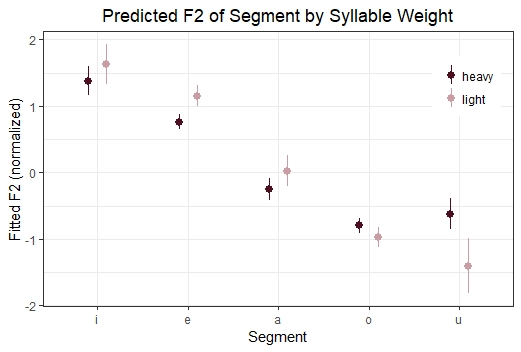
\includegraphics[width=0.75\textwidth]{Figure6.jpg}
    \label{fig:stats_f2_final}
\end{figure}

\newpage

Figure \ref{fig:ellipses_final} shows a visualization of the normalized F1 and F2 of final-syllable vowels. The plot illustrates the general vowel space of each vowel in final syllable based on the weight of the syllable in which it appears. Ellipses are an output of phonR \footnote{PhonR is an R package developed by Daniel R. McCloy. It aids with the analysis of phonetic data and provides the capabilities to create visualizations of the vowel space and formant values.} \citep{mccloy2016} depicting the level of confidence in the location of the mean of each vowel, and they vary in color by syllable weight. One may note that in general, the space each vowel occupies based on weight reflects the model output. Overall, vowels in heavy syllables tend to be more centralized while those in light syllable are more peripheral. The most-dramatic distinction as a result of syllable weight is among mid-vowels. While other segments show little sensitivity to syllable weight, mid-vowels in light syllables have a distinctly lower F1 and occupy a smaller acoustic space than those of mid-vowels occurring in heavy syllables. Tense mid-vowels are so distinct from lax ones that tense mid-vowels occupy roughly the same F1 space as high vowels.

\begin{figure}[h!]
    \centering
    \caption{Mean F1xF2 of final syllable vowels of all speakers. Ellipses show the degree of confidence in the mean F1 and F2 of each. Black ellipses represent vowels in heavy syllables. Gray ellipses represent vowels in light syllables.}
    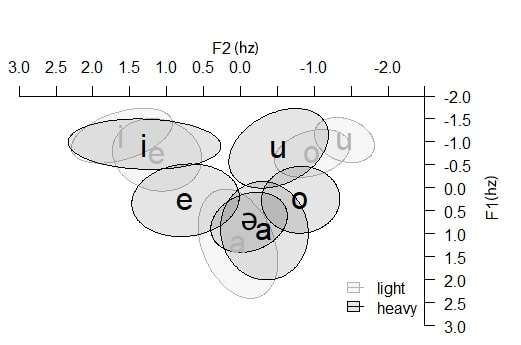
\includegraphics[width=0.75\textwidth]{Figure4.jpg}
    \label{fig:ellipses_final}
\end{figure}

\newpage


The next section details the modeling and outputs regarding vowel harmony, its cause and directionality.

\subsection{Vowel Harmony}\label{sec:harmony}


Tables \ref{tab:Syll2f1_harmony} and \ref{tab:Syll2f2_harmony} display the table of coefficients for the third and fourth LMEM that were employed to observe patterns of vowel harmony in the penultimate syllable. Only the final vowel heights that follow a penultimate mid-vowel were included in the model, thus the absence of high vowels and schwa. The model results confirm that the weight of the penultimate syllable has very little effect on the F1 and the F2 of the penultimate vowel; the interaction between segment and syllable weight in final syllable is not evident in the penultimate syllable (/i/: \textit{t = -0.236 p = n.s.}; /e/: \textit{t = -1.563  p = n.s.}; /a/: \textit{t = 0.250   p = n.s.}; /o/: \textit{t = -0.542  p = n.s}.; /ə/: \textit{t = -0.762  p = n.s.}). \footnote{There were no instances of /u/ in a heavy penultimate syllable and thus the influence of syllable weight on /u/ could not be observed.} Figure \ref{fig:Syll2f1f2_SegWeight} illustrates the F1 and F2 of vowels in penultimate syllables as a result of syllable weight. When compared to Figures \ref{fig:stats_f1_final} and \ref{fig:stats_f2_final}, one may notice that the visual distinction of F1 in mid-vowels and F2 in back vowels is no longer present.

\begin{table}[h!]
\centering
\caption{The table of coefficients for F1 of penultimate syllable vowels. Independent variables include \textsc{segment}, penultimate \textsc{syllable weight}, final syllable \textsc{vowel height}, and \textsc{duration}. There is no effect of syllable weight, and mid-vowels and schwa show most variation as a result of final vowel height.}

\label{tab:Syll2f1_harmony}
%\begin{ruledtabular}
\renewcommand{\arraystretch}{0.5}% Tighter
\begin{tabular}{l | r r r r r}
Effect & Est. & SE & df & t & p-value\\
\hline
(Intercept)          &  1.282  & 0.247  & 32.67    & 5.183   & <.001\\
e                    &  -1.377 & 0.232  & 94.95    & -5.946  & <.001\\
i                    &  -2.795 & 0.368  & 70.20    & -7.597  & <.001\\
o                    &  -1.507 & 0.234  & 83.21    & -4.603  & <.001\\
ə                    &  -8.515 & 0.286  & 123.4    & -2.979  & .000 \\
u                    &  -2.672 & 0.159  & 130.3    & -16.857 & <.001\\
Weightlight          &  -0.042 & 0.166  & 60.81    & 0.250   & .803     \\ 
Height: mid-high     &  -0.079 & 0.142  & 92.68    & 0.561  & .576    \\
Height: mid-low      &  -0.002 & 0.116  & 134.6    & -0.013  & .99    \\
Duration             &  <.001  & <.001  & 1005     & 1.477   & .14 \\
e x Weightlight      &  -0.303 & 0.194  & 80.22    & -1.563  & .122 \\ 
i x Weightlight      &  -0.07  & 0.295  & 54.89    & -0.236  & .814    \\
o x Weightlight      &  -0.112 & 0.206  & 67.77    & -0.542  & .589    \\
ə x Weightlight      &  -0.165 & 0.217  & 102.9    & -0.762  & .448  \\
Height: mid-high x e &  -0.724 & 0.209  & 128.2    & -3.466  & .001\\
Height: mid-high x i &   0.2   & 0.293  & 80.24    & -0.682  & .496  \\  
Height: mid-high x o &  -0.994 & 0.194  & 112.9    & -5.132  & <.001\\
Height:mid-high x ə  &   0.686 & 0.253  & 118.9    & -2.710  & .008   \\
Height: mid-high x u &  -0.086 & 0.391  & 197.6    & -0.220  & .826    \\
Height: mid-low x e  &  -0.281 & 0.178  & 137.6    &  1.580  & .116    \\
Height: mid-low x i  &  -0.085 & 0.248  & 102.5    &  0.344  & .732 \\
Height: mid-low x o  &  -0.309 & 0.164  & 150.9    & -1.888  & .061  \\
Height: mid-low x ə  &  -0.265 & 0.224  & 123.9    & -1.185  & .238    \\
Height: mid-low x u  &  -0.129 & 0.232  & 95.60    & -0.  &555 .58    \\

\end{tabular}
%\end{ruledtabular}
\end{table}

\newpage

\begin{table}[h!]
\centering
\caption{The table of coefficients for F2 of penultimate syllable vowels. Dependent variables include \textsc{segment}, penultimate \textsc{syllable weight}, final syllable \textsc{vowel height}, and \textsc{duration}. There is no effect of syllable weight, and F2 is not influenced by that of the final vowel.}
\label{tab:Syll2f2_harmony}
%\begin{ruledtabular}
\renewcommand{\arraystretch}{0.5}% Tighter
\begin{tabular}{l | l l l l l}
Effect & Est. & SE & df & t & p-value\\
\hline
(Intercept)          &  0.003  & 0.187  & 81.69    & 0.018   & .985\\
e                    &  -0.855 & 0.219  & 88.86    &   3.905 & <.001\\
i                    &  2.23   & 0.353  & 66.48    & 6.324  & <.001\\
o                    &  -0.912 & 0.223  & 78.60    & -4.095  & <.001\\
ə                    &   0.157 & 0.267  & 117.2    &  0.586  & .000 \\
u                    &  -1.059 & 0.148  & 125      & -7.166 & <.001\\
Weightlight          &  -0.173 & 0.16   & 56.86    & -1.082  & .284     \\ 
Height: mid-high     &  -0.046 & 0.134  & 87.69    & -0.345  & .731    \\
Height: mid-low      &  -0.021 & 0.108  & 132.7    & -0.193  & .847    \\
Duration             &  <.001  & <.001  & 613.3    & -1.662  & .097 \\
e x Weightlight      &   0.256 & 0.185  & 74.85    &  1.387  & .17 \\ 
i x Weightlight      &   0.063 & 0.286  & 50.74    &  0.221  & .826    \\
o x Weightlight      &  -0.004 & 0.198  & 63.82    & -0.022  & .983    \\
ə x Weightlight      &  -0.007 & 0.204  & 92.76    &  0.323  & .747  \\
Height: mid-high x e &   0.302 & 0.195  & 123.3    &  1.549  & .124 \\
Height: mid-high x i &  -0.235 & 0.278  & 77.98    & -0.845  & .401  \\  
Height: mid-high x o &  -0.035 & 0.182  & 109      & -1.192  & .848 \\
Height: mid-high x ə &   0.134 & 0.237  & 119.6    &  0.567  & .572   \\
Height: mid-high x u &  -0.318 & 0.361  & 156      & -0.88   & .38    \\
Height: mid-low x e  &  -0.126 & 0.165  & 133      &  0.777  & .438    \\
Height: mid-low x i  &  -0.36  & 0.233  & 105.8    & -1.541  & .126 \\
Height: mid-low x o  &  -0.153 & 0.152  & 149.3    &  1.006  & .316  \\
Height: mid-low x ə  &  -0.195 & 0.209  & 125.4    & -0.933  & .352    \\
Height: mid-low x u  &  -0.17  & 0.219  & 91.76    & -0.776  & .439   \\

\end{tabular}
%\end{ruledtabular}
\end{table}

\newpage

\begin{figure}[h!]
    \centering
    \caption{F1 and F2 model outputs of penultimate segments as influenced by penultimate syllable weight. Segments no longer show sensitivity to syllable weight.}
    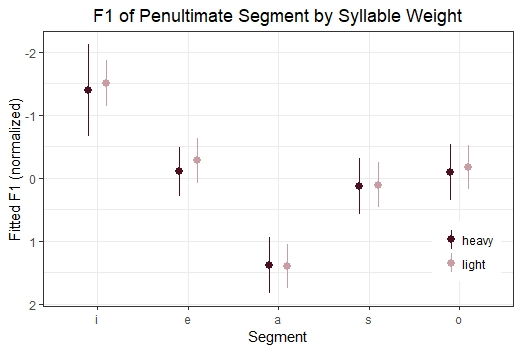
\includegraphics[width=0.75\textwidth]{Figure7.jpg}
    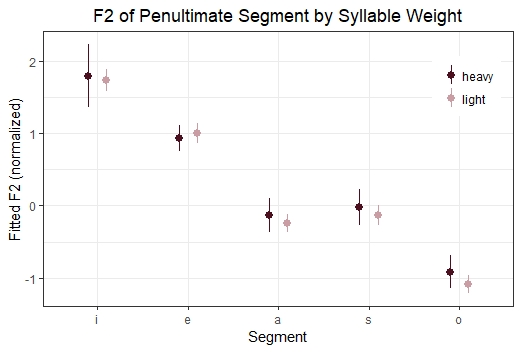
\includegraphics[width=0.75\textwidth]{Figure8.jpg}
    \label{fig:Syll2f1f2_SegWeight}
\end{figure}

\newpage


Model results also reveal that the height of the vowel in the final syllable influences the formant values of penultimate mid-vowel segments. Figures \ref{fig:Syll2f1_Segfh} and \ref{fig:Syll2f2_Segfh} exhibit the mean formant values for each penultimate segment based on the height of the following vowel. The patterns in this figure are similar to those in \ref{fig:stats_f1_final} and \ref{fig:stats_f2_final} in that there is a visible difference between mid-vowels that precede a tense mid-vowel and mid-vowels that precede a lax mid-vowel or /a/. The model output demonstrates that both front mid-vowels and back mid-vowels are significantly different (e x mid-high vowel: \textit{t = -3.466  p = .001}; o x mid-vowel : \textit{t = -5.132  p = <.001}). Schwa shows this same pattern as front mid-vowels (\textit{t = -2.710  p = .008}). Although duration is included as a factor in the model, conclusions about schwa should still be regarded skeptically. The average length of schwa in penultimate syllable is 76 ms in contrast to the 156 ms average of other vowels. Such a short voicing duration causes more variability in the pronunciation of the utterance because it takes on more of the properties of the adjacent consonant \citep{lindblom1963}. Formant values of low and high vowels do not appear to rely on the height of the following vowel.
 
\begin{figure}[h!]
\centering
    \caption{F1 of penultimate segments as influenced by final syllable height. "Mid-high" refers to [e] and [o] in final syllable while "mid-low" refers to [ɛ] and [ɔ] in final syllable. Mid-vowels including schwa show the greatest effects. F1 is higher when preceding low mid-vowels or /a/.}
    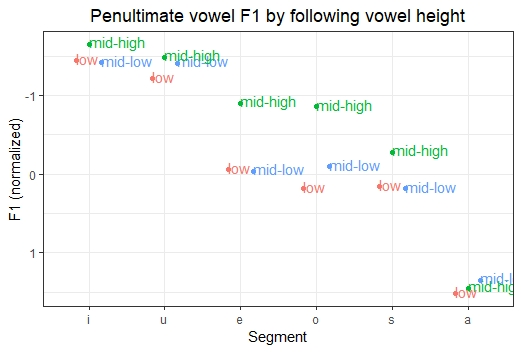
\includegraphics[width=0.75\textwidth]{Figure9.jpg}
    \label{fig:Syll2f1_Segfh}
\end{figure}


\begin{figure}[h!]
\centering
    \caption{F2 of penultimate segments as influenced by final syllable height. "Mid-high" refers to [e] and [o] in final syllable while "mid-low" refers to [ɛ] and [ɔ] in final syllable. Mid-vowel F2 does not vary as a result of final syllable height.}
    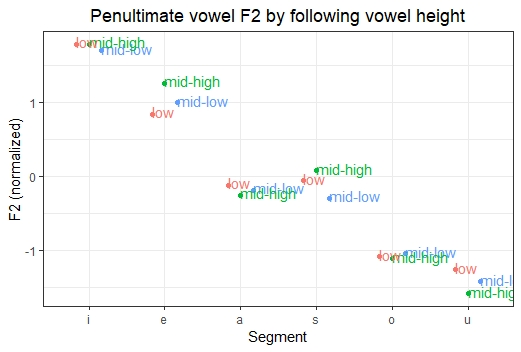
\includegraphics[width=0.75\textwidth]{Figure10.jpg}
    \label{fig:Syll2f2_Segfh}
\end{figure}

The F2 of the penultimate vowel does not show any sensitivity to that of the final vowel. This is unsurprising since harmony appears to be driven by height and not backness.

\newpage

\section{Discussion}\label{sec:discussion}

This study aimed to answer two pertinent questions: 1) Can variations in mid-vowels in final position be explained by differences in syllable weight? and 2) Are penultimate vowels also sensitive to syllable weight, and to what extent are they sensitive to the quality of the vowel in the final syllable?
The presented results address the first question by showing that in final syllables, syllable weight drives vowel-quality. Results show that final syllable mid-vowels were higher in light syllables than in heavy syllables. Word-final back vowels were lower in light syllables than in heavy syllables. In response to the second question, syllable weight does not influence the vowel in penultimate syllables. Results revealed no variation among vowels in heavy vs. light penultimate syllables. Instead, the quality of penultimate mid-vowels is driven by the quality of the final vowel. Penultimate mid-vowels were higher when preceding high mid-vowels. They were lower when preceding low mid-vowels or /a/. 

These results suggest that variation between Ampenan Sasak [e]~[ɛ] and [o]~[ɔ] is largely predictable. In final syllables, the weight of the syllable affects the realization of the vowel. In syllables with a non-glottal stop coda [e] and [o] are produced as [ɛ] and [ɔ]. The results also indicate that vowel harmony is occurring among mid-vowels in penultimate syllable. The weight of the penultimate syllable does not have the same effect on the F1 and F2 of the penultimate vowel as it does in the final syllable. Rather, it is the F1 of the vowel in the final syllable that influences realization of the penultimate syllable. These effects are strongest among mid-vowels including schwa. Mid-vowels /e/ and /o/ and schwa lower when the following mid-vowel lowers in a closed syllable or when preceding a low vowel. 

In contrast to \citet{chahal1998} who observed bi-directional height harmony in the Meno-mene variety of Sasak, the vowel harmony observed in Ampenan Sasak appears to be unidirectional. The vowel in the final syllable can influence the penultimate syllable vowel in Ampenan Sasak, but left-to-right harmony does not occur. Because there were no effects of penultimate syllable weight on the penultimate vowel, it is implausible that the features of the penultimate vowel would spread rightward.  Thus, it appears that Sasak has right-to-left height harmony, which most-robustly affects mid-vowels including schwa. This type of vowel harmony in Sasak does not appear to be unusual among the languages of this region. Javanese has nearly the same phenomenon \citep{adisasmito1999}. In Javanese, vowels in final syllable are generally tense in open syllables and lax in closed syllables. In eastern Javanese, when vowels are the same height and backness, a vowel in a light penultimate syllable laxes to match the lax vowel in the final syllable. In central Javanese, this harmony only occurs among mid and low-vowels.

As noted previously, stress is a contested topic in the region, and Sasak's stress remains elusive. If stress were to play a role on vowel quality, it may interact with the current results in several ways, but none would have significant influence on the results presented here. Firstly, if Sasak had fixed phrase-level stress each word of interest would have equal stress since each word occurred word-initially. Similarly, if there was fixed word-level stress, because this study would thus only compare syllables of equal stress (final with final and penultimate with penultimate). If stress were variable within the word, its effect would depend on the nature of this variability. If heavy syllables were stressed, then under the current study, it would be impossible to tease apart whether the driving factor for vowel quality is syllable weight or stress. Regardless, it does not disregard the observation that mid-vowels lower in heavy syllables. There is also the possibility that final syllables are only stressed if heavy and otherwise the penultimate vowel is stressed, which is already accounted for in this analysis. The nature of coding for harmony of the penultimate vowel took syllable weight (or stress) into account: `mid-high' vowels only occur in light or unstressed final syllables and `mid-low' vowels only occur in heavy or stressed final syllables. Because of the nature of the data, there are no other instances where syllable weight might affect the results since this is the only environment where final weight may have an influence; otherwise mid-vowels never occur before high vowels, and front vowels only occurred before /a/ in light syllables and back vowels only before /a/ in heavy syllables. These restrictions are, admittedly, a weakness of the current dataset and should be addressed in future studies. Thus, while stress thus does not nullify the current results, this study has revealed the need for a stress study of Sasak in order to fully understand the language's phonological and typological contributions.

It must be noted that there are several limitations to this study. Firstly, Sasak is an under-documented language and the data is limited. It is probable that researchers have not yet identified all vowel contexts. It is also quite likely that researchers have not yet identified all minimal or near-minimal pairs between mid-vowels.  Further, this study focuses on the distribution of mid-vowels in Sasak. As a result, the administered wordlist does not identify or include exhaustive environments of high vowels /i/, /u/, or schwa. Any claims made about the distribution and patterns observed among high vowels in particular require more data to be confirmed. 

Nevertheless, this acoustic data suggests that mid-vowels in Ampenan Sasak are largely predictable based on final syllable weight. Thus, in conjunction with elicitation data, which shows several clear minimal pair among back mid-vowels, they may be considered to be in a ``just barely contrastive'' relationship; they are almost entirely predictable with some exceptions \citep[10]{goldsmith1995}. As the results of this study suggest, one can identify distinct conditioning environments (e.g., syllable weight and the height of the following vowel) that influence whether mid-vowels are produced as tense or lax. Yet, the occasional minimal pair between back mid-vowels and the phonotactics of borrowings provide notable exceptions to these trends. 

This is just one of many possible intermediate phonological (or quasi-phonemic) relationships that may exist between segments. The ``just barely contrastive '' relationship between Ampenan Sasak mid-vowels is most-similar to Canadian raising. In Canadian English as well as varieties of English outside of Canada, such as Philadelphia English, the diphthongs [ɑɪ], [ɑʊ],[ʌɪ], and [ʌʊ] are largely predictable with a few exceptions. Generally [ʌɪ], and [ʌʊ] occur before voiceless segments while [ɑɪ], [ɑʊ] occur in other environments. As a result, predictable minimal pairs such as `tight' and `tide' exist. However, there are several near-minimal pairs between the two sets of diphthongs that break this paradigm and are otherwise unexplainable. These include `spider' [spʌɪɾɚ] versus `cider' [sɑɪɾɚ] and `espouse' [ɛspʌʊz] versus `houses' [haʊzəz] \citep{myers1993}. Similarly, in Pulaar, some mid vowels are retracted unless they occur before an advanced vowel (usually a high vowel), in which case they become advanced. But there are a few mid advanced suffixes (which have no following advanced vowel). The patterns in these languages are similar to Sasak in that there is a regular allophonic rule, with some sporadic lexical exceptions which cannot be neatly explained. 

While some authors would conclude that Ampenan Sasak mid-vowels are necessarily phonemes as a result of their marginal yet notable minimal and near-minimal pairs, this study follows \citet[15]{scobbie2008} who, in their analysis of Scottish English diphthongs, state, ``We thus do not offer a solution to the question of whether /ai/ is one member of the inventory of [Scottish Standard English] or two. One reason for this is that we hope to leave the reader with the same sense of unease which we feel about the requirement to adopt one ill-fitting and rigid phonological analysis over another.” Echoing these closing sentiments, this paper does not present a definitive conclusion as to whether Ampenan Sasak mid-vowels are phonemes or allophones. In fact, considering the data, categorizing them as such is impossible. Instead this paper explicitly classifies them as quasi phonemes. As more studies identify probabilistic nature of many phonemic contrasts, it is becoming clear that `phonemes' and `allophones' should not be the only possible categorizations for segments in a language's inventory. Recent advances in phonological theory support this hesitation as well. 

In recent decades, phonological theories of discrete symbols have been altered or replaced by theories that acknowledge the variability and the gradience within the phoneme and the phonological inventory as a whole. \citet{smolensky2016} in their recent development of Gradient Symbolic Representations propose gradience within the discrete phoneme. Others such as \citet{hall2009,hall2012,hall2013} propose ways to account for gradience within the phonological inventory. Additionally, Exemplar Theory is built upon the idea that both speech and representations are continuous and highly variable \citep{goldinger1998, johnson2005} thus allowing “messy and ambiguous facts to percolate into analyses better than many [other theories]” \citep[16]{scobbie2008}. Each theory has been born of instances in which a phonological theory of discrete phonemes does not suffice and an incorporation of gradience is necessary to describe real-world phenomena. As these theories progress and nearly-universally call for a recognition of gradience within phonology, it suggests that for instances such as that described in this paper, it is unnecessary to categorize all segments as phonemes or allophones. 

While not all languages have quasi-phonemes, their existence have been identified in enough languages --- e.g. Scottish English, Canadian English, Spanish, Texhuacan, and Mandarin --- to suggest their widespread occurrence. It may thus be reasonable to assume that intermediate segments are widespread throughout the world's languages. This paper does not necessarily suggest that quasi-phonemes be integrated into grammars; categorization can be useful for language description purposes. However, a recognition that some segments cannot be categorized may help researchers who are trying to adequately describe an under-documented language's phonemic inventory, both regular and idiosyncratic. If indeed, quasi-phonemes are a common occurrence, a simple recognition of their existence may help further future research in phonological theory as more situations are described.

In the context of Sasak, the  conclusions of this paper suggest that the distribution of Ampenan Sasak mid-vowels is distinct from previous acoustic studies of Sasak. Not only are the predictable environments different from those observed by \citet{chahal1998} and \citet{archangeli2018}, but the fact that /ʔ/ coda patterns as a light syllable is also distinct. Further study of Sasak mid-vowels may also reveal information about the nature of borrowed words or about a current phoneme inventory shift in Sasak. The avoidance of designating the phonemes that make up Ampenan Sasak's vowel inventory should encourage future researchers to more-openly consider the possibility of quasi-phonemes or other segments who exhibit gradience, particularly in under-documented languages.

% Linguists who aim to identify the phonetic or phonological patterns of an under-documented language should be aware of the nuances that exist and should strive to include such nuance in their grammatical descriptions. Doing so will help future researchers identify areas for study to untangle the more puzzling areas of phonetic and phonological description. 

% %% before appendix (optional) and bibliography:
% \begin{acknowledgments}
% I thank all of the speakers who kindly participated in this study as well as Khairunnisa and family, Bradley McDonnell, and Rory Turnbull for their support. This study was funded by the Bilinski Foundation.
% \end{acknowledgments}

\section*{References}
\bibliography{pappas}
\newpage

\section*{Appendix A: Wordlist}

\begin{table}[]
    \centering
    \begin{tabular}{c|l l l}
    Coda Segement & Sasak & Indonesian & English  \\
    \multirow{4}{*}{q} & bembeq & kambing & goat\\
                       & cendeq & pendek & short\\
                       & tabeq & permisi & excuse me\\
                       & kodeq & kecil   & small \\
    \hline
    \multirow{4}{*}{h} & bareh & kemudian & later\\
                       & teteh & buang & throw away\\
                       & jangkeh & kompor & stove\\
                       & biweh & mulut   & mouth \\
    \hline                   
    \multirow{2}{*}{n} & angen  & perasaan & feeling\\
                       & duren & durian & durian\\
    \hline                   
    \multirow{4}{*}{ng} & goreng & goreng & fried\\
                       & peteng & gelap & dark\\
                       & adeng & pelan & slowly\\
                       & kepeng & uang   & money \\
    \hline                   
    \multirow{3}{*}{p} & tutep & dekat & close\\
                       & sangkep & pipi & cheek\\
                       & kelep & terbang & fly\\
    \hline                   
    \multirow{4}{*}{t} & deket & dekat & near\\
                       & silet & cutter & silet\\
                       & anget & mengunya & chew\\
                       & kocet & kecil   & small \\
    \hline                   
    \multirow{2}{*}{s} & peles & toples & jar\\
                       & tedes & semut & ant\\
                       & ampes & ?     & ? \\
    \hline
    \multirow{2}{*}{l} & mehel & mahal & expensive\\
                       & model & model   & model \\
    \hline 
    \multirow{4}{*}{r} & teker & petir & lightning\\
                       & jengger & ? & rooster comb\\
                       & ceker & ceker & chicken feet\\
                       & jelamer & bibir   & lip \\
    \hline
    \multirow{3}{*}{k} & potek & mentah & unripe fruit\\
                       & bebek & bebek & duck\\
                       & kerek & kulit yang kering & bumpy skin\\
    \hline
    \multirow{3}{*}{0} & tape & tapai & edible fermented rice\\
                       & sere & serai & lemongrass\\
                       & geroge & kepiting pasir & k.o. crab\\
    \end{tabular}
    \caption{Words with penultimate 'e'}
    \label{tab:my_label}
\end{table}

\begin{table}[]
    \centering
    \begin{tabular}{c|l l l}
    Coda Segement & Sasak & Indonesian & English  \\
    \hline
    \multirow{3}{*}{k} & gubok & desa & village\\
                       & kapok & melempar & throw at something\\
                       & bolok & mata & mata\\
    \hline
    \multirow{4}{*}{q} & jonjoq & memberikan & give by hand\\
                       & seboq & menyembunyikan & hide\\
                       & bisoq & mencuci & wash\\
                       & bokoq & bengkak   & swollen \\
    \hline
    \multirow{4}{*}{n} & sigon & wajan & wok\\
                       & semeton & saudara kandung & sibling\\
                       & molon & halus, polos & bald\\
                       & akon & diadopsi   & adopted \\
    \hline
    \multirow{4}{*}{ng} & jagong & jagung & corn\\
                       & kotong & gosong & burnt\\
                       & kedong & tidak mungkin & not possible\\
                       & idong & hidung   & nose \\
    \hline
    \multirow{4}{*}{t} & tinjot & terkejut & surprised\\
                       & kentot & pendek & too short\\
                       & bacot & tenggorokan & throat\\
    \hline
    \multirow{3}{*}{s} & kemos & tersenyum & smile\\
                       & empos & pukulan & to blow\\
                       & bokos & kafan & funeral cloth\\
    \hline
    \multirow{2}{*}{r} & kocor & ketel & kettle\\
                       & embor & embun & dew\\
    \hline
    \multirow{3}{*}{l} & kecimol & kecimol & k.o. music\\
                       & tongkol & tongkol & mackerel tuna\\
                       & tokol & duduk & sit\\
    \hline
    \multirow{3}{*}{h} & betijoh & meludah & spit\\
                       & galoh & lebar & wide\\
                       & bognoh & baik & good?\\
    \hline
    \multirow{4}{*}{0} & kado & rugi & lose money\\
                       & rebo & rabu & Wednesday\\
                       & poto & ujung & tip\\
                       & kolo & perkutut & k.o. dove\\

    \end{tabular}
    \caption{Words with penultimate 'o'}
    \label{tab:my_label}
\end{table}

\begin{table}[]
    \centering
    \begin{tabular}{c|l l l}
    Coda Segement & Sasak & Indonesian & English  \\
    \multirow{4}{*}{filler} & berempokan & bertabrakan & collide\\
                       & ompal & mengapung & float\\
                       & tipah & tikar & traditional mat\\
                       & sukah & sulit   & difficult \\
                       & otak & kepala & head, brain\\
                       & pedis & asam & sour\\
                       & ladik & pisau & knife\\
                       & bari & basi & ?\\
                       & nasiq & nasi & cooked rice\\
                       & sikuq & siku & elbow\\
                       & batur & teman & friend\\
                       & idup & hidup & life\\
                       & kuning & kuning & yellow\\
                       & beaq   & merah & red\\
                       & 
    \end{tabular}
    \caption{Filler segments}
    \label{tab:my_label}
\end{table}

\end{document}
